\section{Method}
Here the methodology and equipment choices of the performed experiments are described. The logical place to begin is with the silicon chips, which are the central object of interest in the experiments. The following three chips were used throughout the investigation:
\begin{itemize}
	\item {\bf Toshiba } 
	\item {\bf Glassgow }
	\item {\bf HP }
\end{itemize}


In order to perform experiments on silicon photonic chips a way to couple light from a fiber optic cable must be established. There exist a few ways to achieve this, here we used lens fibers to focus light onto a region of the chip designed for coupling. 
\subsection{Collecting a JSI}
\begingroup
    \centering  
    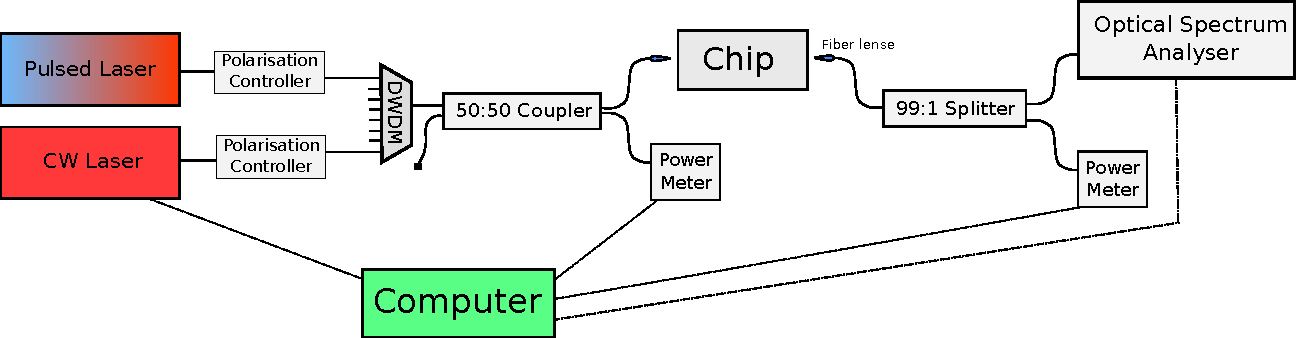
\includegraphics[width=18cm]{img/method/setup_1.pdf}
    \captionof{figure}{Glassgow test structure chip}
     \vspace{3pt} \label{crossCompare}
\endgroup

\begingroup
    \centering  
    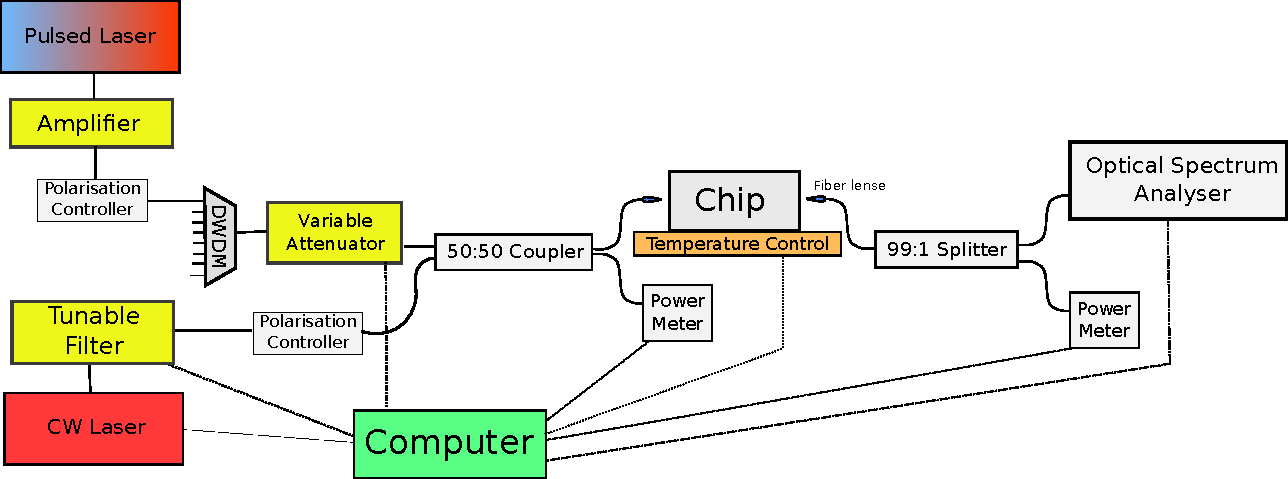
\includegraphics[width=18cm]{img/method/setup_2.pdf}
    \captionof{figure}{big experiment}
     \vspace{3pt} \label{crossCompare}
\endgroup
\begingroup
    \centering  
    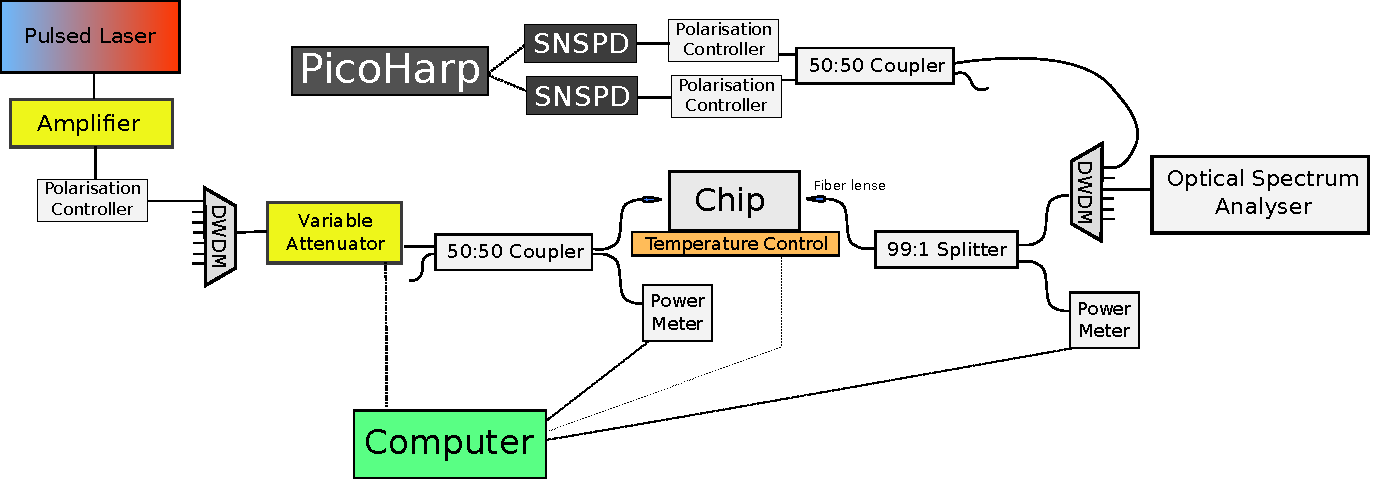
\includegraphics[width=18cm]{img/method/setup_3.pdf}
    \captionof{figure}{single photon}
     \vspace{3pt} \label{crossCompare}
\endgroup

\subsection{Silicon Chips}
\subsubsection{Glassgow}
\begingroup
    \centering  
    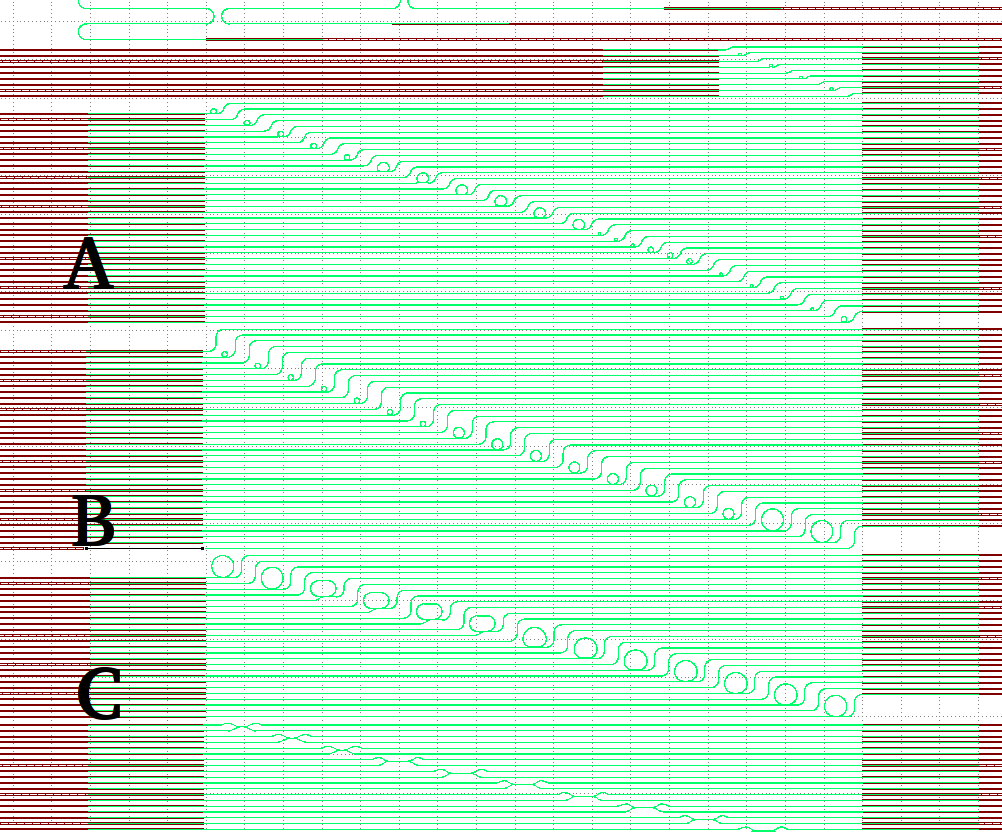
\includegraphics[width=10cm]{img/method/glassgowChipNumbering.png}
    \captionof{figure}{Glassgow test structure chip}
     \vspace{3pt} \label{crossCompare}
\endgroup
\subsubsection{Toshiba}
\begingroup
    \centering  
    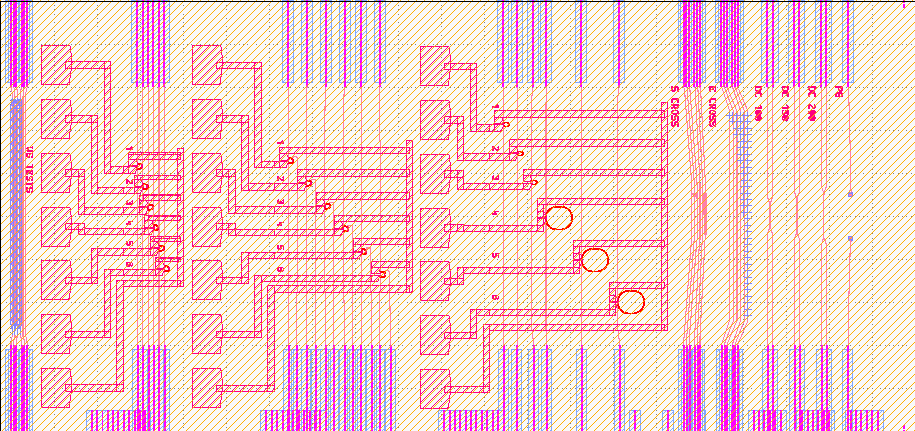
\includegraphics[width=10cm]{img/method/toshiba.png}
    \captionof{figure}{Glassgow test structure chip}
     \vspace{3pt} \label{crossCompare}
\endgroup
\subsubsection{a-Si}
\begingroup
    \centering  
    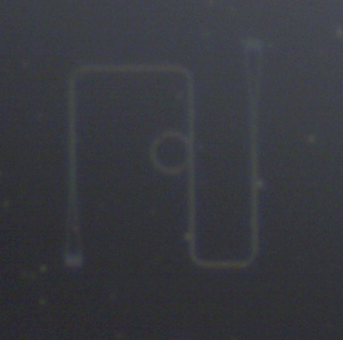
\includegraphics[width=10cm]{img/method/chipPictures/exampleASIRing.png}
    \captionof{figure}{Glassgow test structure chip}
     \vspace{3pt} \label{crossCompare}
\endgroup
\subsection{Coupling}
% Side/Vertical coupling
% Coupling loss
% Blowing up chips -> tempted to add this as a complaint
%	Particularly on glassgow chip
% Temperature tuning
\subsection{Joint Spectrum}
Take the convention that the {\bf signal} photon is the one we measure and the {\bf idler} is the one we stimulate.
% OSA Resolution discussion might be important. Because I think it might have skrewed me over somewhat.
% Filtering
% Could reference the model so that I don't have to use example data.
\subsection{What experiments can be done?}
Assuming from the above that the procedure for collecting the JSI is fixed and fully understood the question that now needs to be answered is: what parameters can be reliably varied to change the JSI?
One that we pursue and that forms the main part of this work is varying the power of the pump laser injected into the ring. This is of interest as it may 
\subsection{$g^{(2)}(0)$}
% Breif description of how this works.
\subsection{Analysing Data}
% The algortihm reflects how using narrow filters increases the purity well
% SNR
% NOISE
% NORALISATION
% SPM
% RING DEFORMATION
% How to calculate Q, r, tau
% Comparing with the simulation

% I want to really discuss what we can hope to keep constant and what we can vary. Where you need to really do som engineering to get insights.